\section{Reanalysis of bow shock sources from Kobulnicky et al. (2016,
  2017, 2018)}
\label{app:bow-shock-data}

In a series of papers \citeauthor{Kobulnicky:2018a} provide an
extensive mid-infrared-selected sample of over 700 candidate stellar
bow shock nebulae (\citealp{Kobulnicky:2016a, Kobulnicky:2017a,
  Kobulnicky:2018a}, hereafter K16, K17, and K18).  For 20 of these
sources, reliable distances and spectral classifications are provided
(Table~5 of K17 and Tables~1 and~2 of K18), and these are used in
\S~\ref{sec:summary-discussion}, where we discuss the
\(\tau\)--\(\eta\) diagnostic diagram.  In this appendix, we outline our
treatment and analysis of the data in these catalogs, which differs in
some important respects from that of the original authors.

The UV optical depth of the bow shell is obtained
(eq.~[\ref{eq:tau-empirical}]) from the ratio of infrared shell
luminosity to stellar luminosity.  The inverse of this ratio is given
in Table~5 of K17, but we choose to re-derive the values since the
spectral classification of some of the sources was revised between K17
and K18.  Although K17 found the total shell fluxes from fitting dust
emission models to the observed SEDs, we adopt the simpler approach of
taking a weighted sum of the flux densities \(F_\nu\) (in \si{Jy}) in
three mid-infrared bands:
\begin{multline}
  \label{eq:total-ir-flux}
  F_{\text{IR}}  \approx \bigl[  2.4\,(F_8 \text{ or } F_{12})
    + 1.6\,(F_{22} \text{ or } F_{24})  \\
  + 0.51\,F_{70}\bigr]
  \,\times \SI{e-10}{erg.s^{-1}.cm^{-2}} \ ,
\end{multline}
where \(F_8\) is Spitzer IRAC \SI{8.0}{\um}, \(F_{24}\) is Spitzer
MIPS \SI{23.7}{\um}, \(F_{12}\) and \(F_{22}\) are WISE bands 3 and 4,
and \(F_{70}\) is Herschel PACS \SI{70}{\um}.  The weights are chosen
so that the integral \(\int_0^\infty F_\nu \,d\nu\) is approximated by the sum
\(\Sigma_k F_k\, \Delta\nu_k\), under the assumption that fluxes in shorter (e.g.,
IRAC \SI{5.8}{\um}) and longer (e.g., PACS \SI{150}{\um}) wavebands
are negligible.  Shell fluxes are converted to luminosities using the
assumed distance to each source, and stellar luminosities are taken
directly from K18 Table~2, based on spectroscopic classification and
the calibrations of gravity and effective temperature from
\citet{Martins:2005a}.  

\begin{figure}
  \centering
  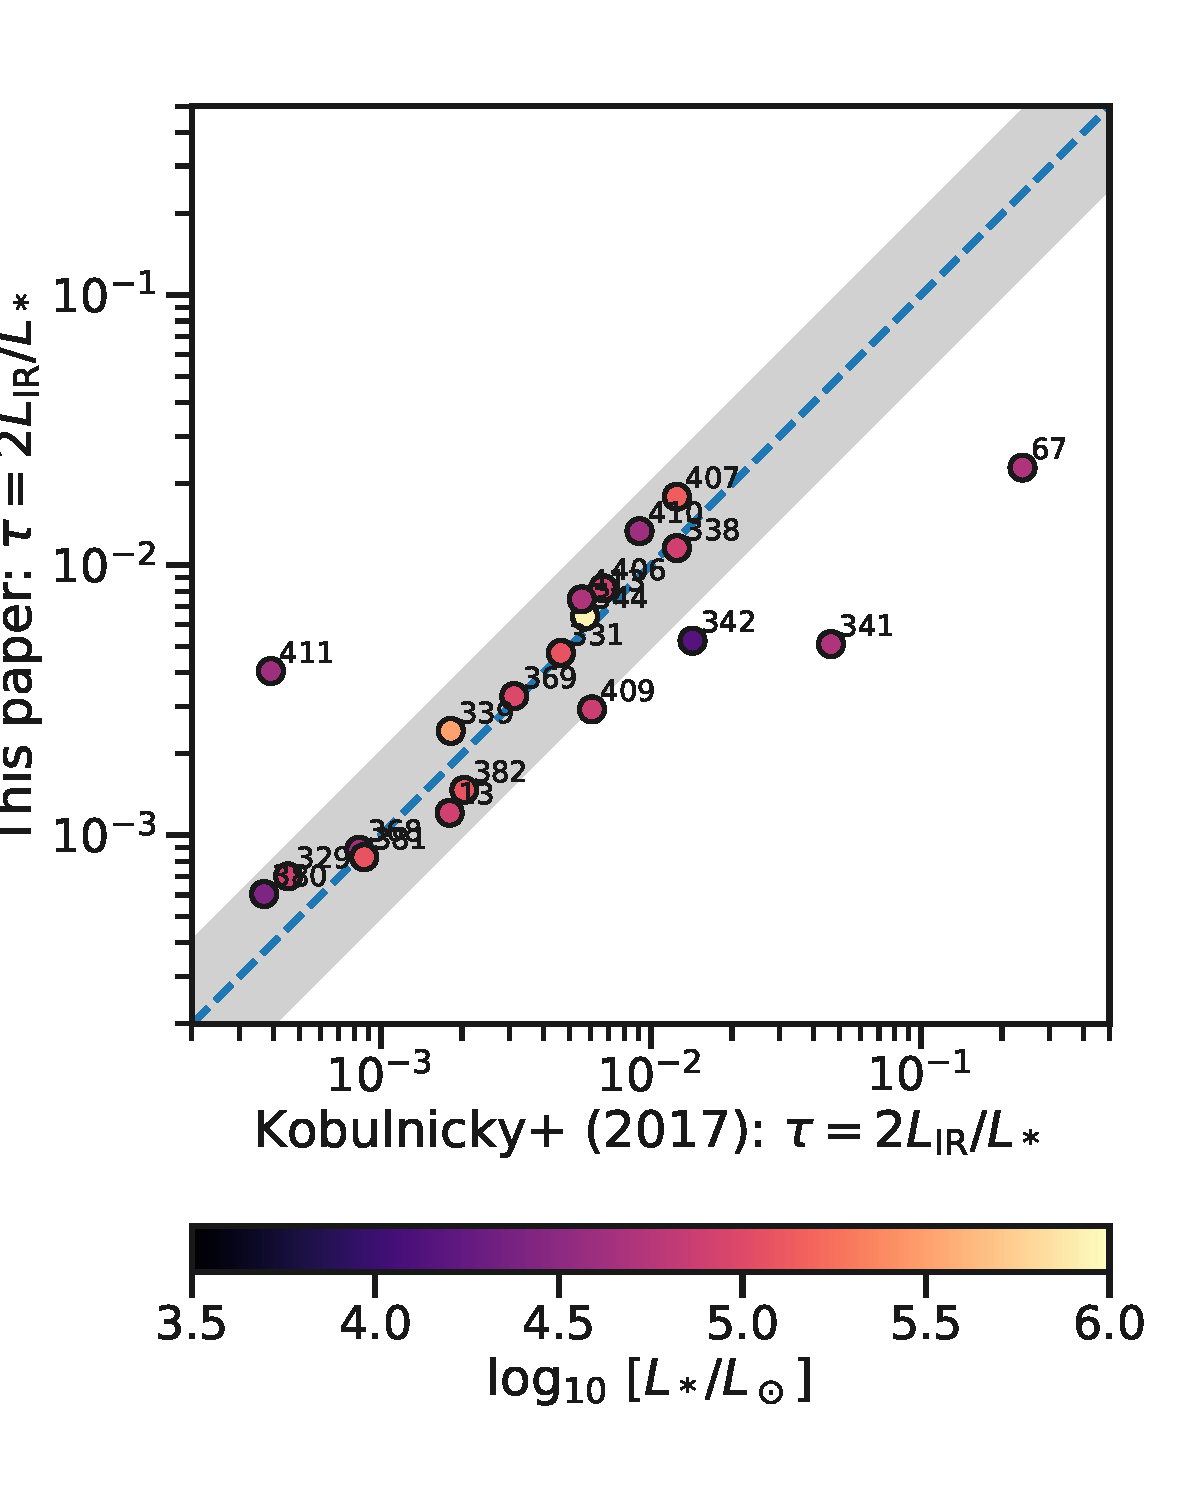
\includegraphics[width=\linewidth]{figs/K17-tau-comparison}
  \caption{Comparison between shell-to-star luminosity ratios
    calculated in the text (\(y\) axis) with those given in K17 (\(x\)
    axis).  The blue dashed line signifies equality and the gray band
    shows ratios between 1/2 and 2.}
  \label{fig:k17-k18-comparison}
\end{figure}

In Figure~\ref{fig:k17-k18-comparison} we compare the \(\tau\) obtained
using the shell luminosity as described above with that obtained using
the luminosity ratios directly from K17 Table~5.  It can be seen that
for the majority of sources the two measurements are consistent within
a factor of two (gray band).  The three furthest-flung outliers can be
understood as follows:
\begin{description}
\item[\textit{Source 67}] This has a very poor-quality spectral fit in
  K17 (see lower left panel of their Fig.~12) and so the
  \(F_{\text{IR}}\) is overestimated by a factor of 10.
\item[\textit{Sources 341 and 342}] The spectral classes changed from
  B2V in K17 to O9V and B1V, respectively, in K18, increasing the
  derived \(L_*\), which lowers \(\tau\).
\item[\textit{Source 411}] The luminosity class changed from Ib (K17)
  to V (K18), so \(L_*\) has been greatly reduced, which increases
  \(\tau\).
\end{description}



% So everything looks OK, except:

% * Source 67 is over 10 times too bright in the Kobulnicky table

% So, I will use my fluxes instead.  

% \begin{figure*}
%   \centering
%   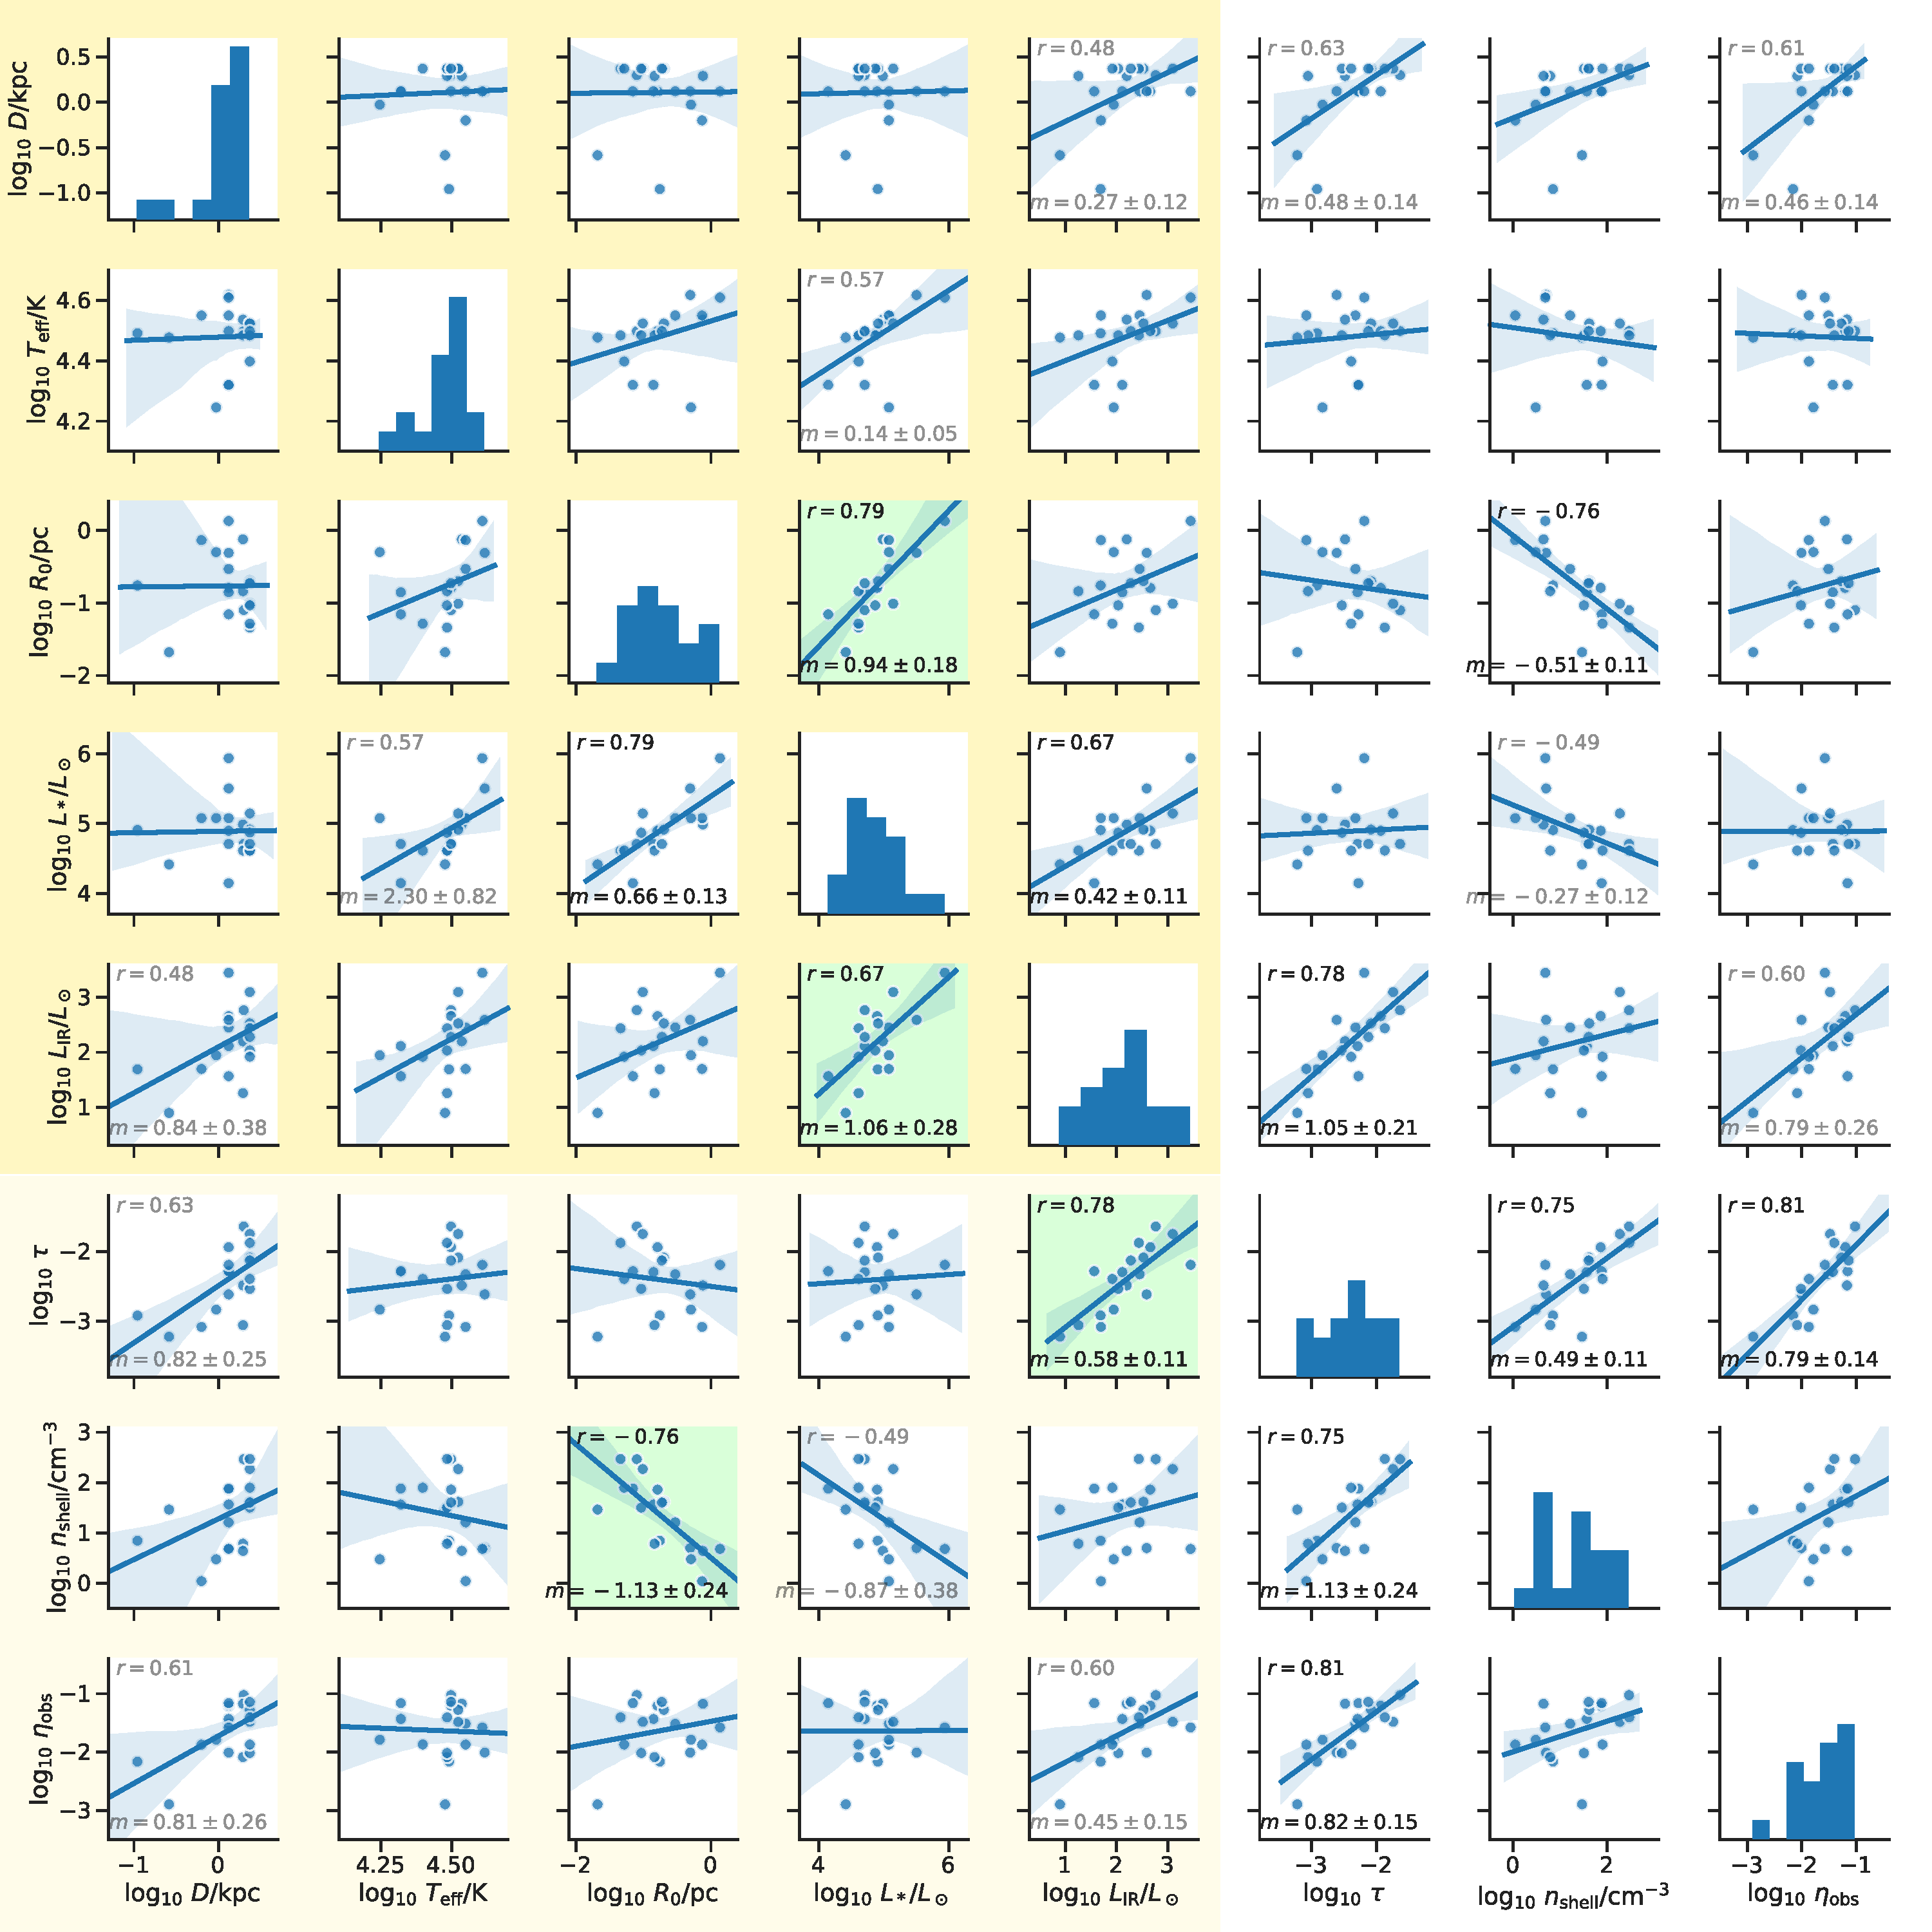
\includegraphics[width=\linewidth]{figs/K18-pairplot-edited}
%   \caption[K18 pair plot]{Pair plots of correlations between observed
%     and derived parameters of bows from the \citep{Kobulnicky:2018a}
%     sample.}
%   \label{fig:K18-pairplot-edited}
% \end{figure*}


% In this graph we compare the original luminosity ratio taken directly from the Kobulnicky (2017) table (x axis) with the ratio calculated using my new total IR fluxes, combined with the new luminosities in the Kobulnicky (2018) table (y axis).   Most of the points show reasonable agreement between the two methods, with a few exceptions:

% * 67: this had the $F_\text{IR}$ overestimated in K17.  Using a more reasonable value gives a lower $\tau$
% * 341: The spectral class has changed from B2 (K17) to O9 (K18), increasing the assumed $L_*$, which lowers $\tau$
% * 411: The luminosity class has changed from Ib (K17) to V (K18), so $L_*$ has been greatly reduced, which increases the estimated $\tau$

% And there doesn't seem to be any significant correlation with stellar luminosity.


\begin{figure}
  \centering
  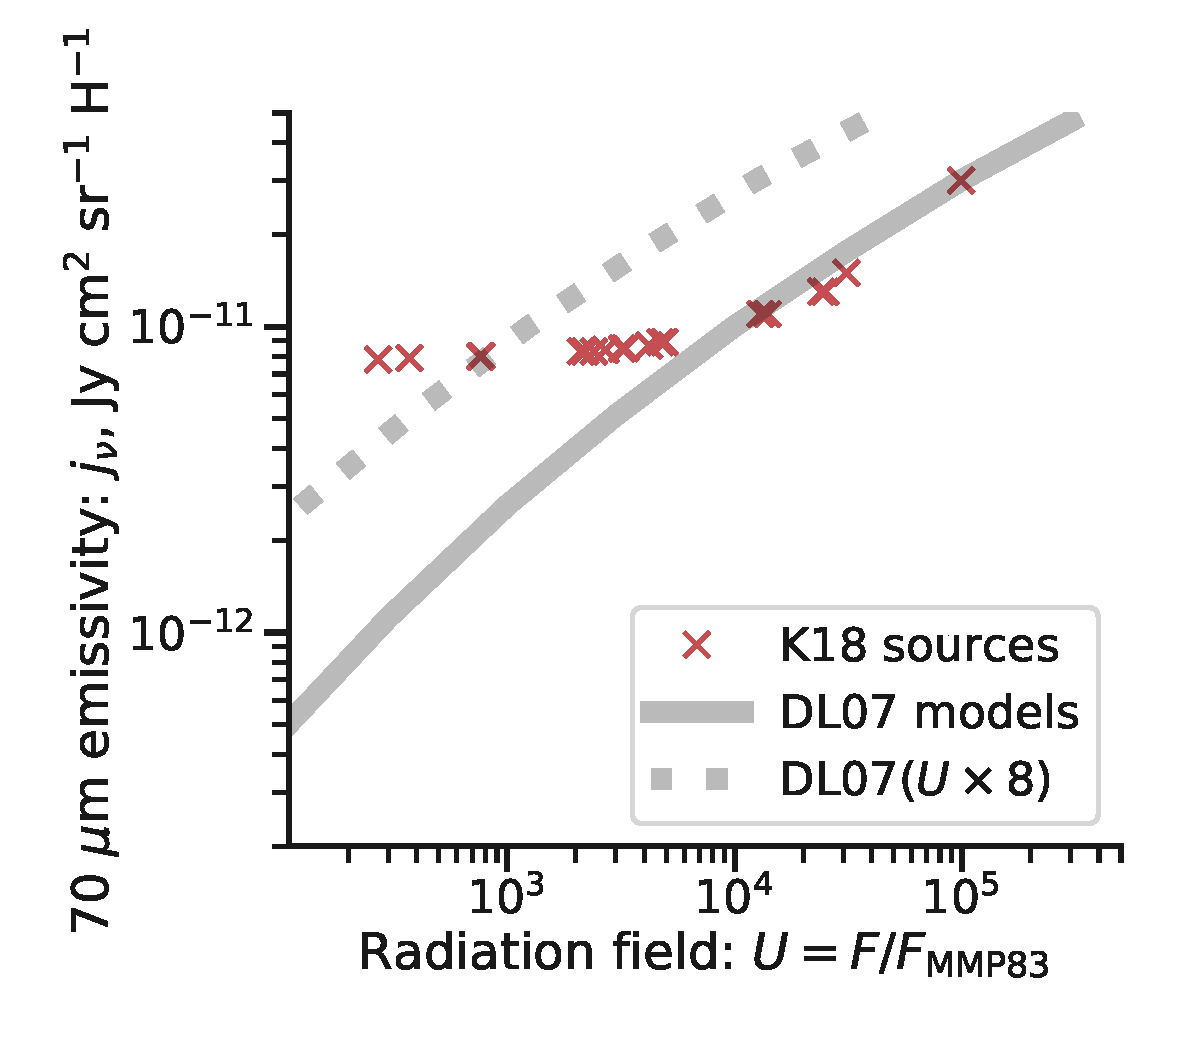
\includegraphics[width=\linewidth]{figs/K18-emissivity-vs-U}
  \caption{Discrepancies in \SI{70}{\um} emissivities that we have
    identified in K18.  Red crosses show the emissivities given in
    K18's Table~2 as a function of the radiation field \(U\), while
    the solid gray line shows the emissivities that they claim to be
    using from \citet{Draine:2007a}.  The dashed line shows the
    emissivities that we believe they should have been using, which
    correct for the fact that the illuminating SED in
    \citet{Draine:2007a} is dominated by longer wavelengths (see
    App.~\ref{sec:grain-temp-emiss}).}
  \label{fig:k18-emissivity}
\end{figure}

\begin{figure}
  \centering
  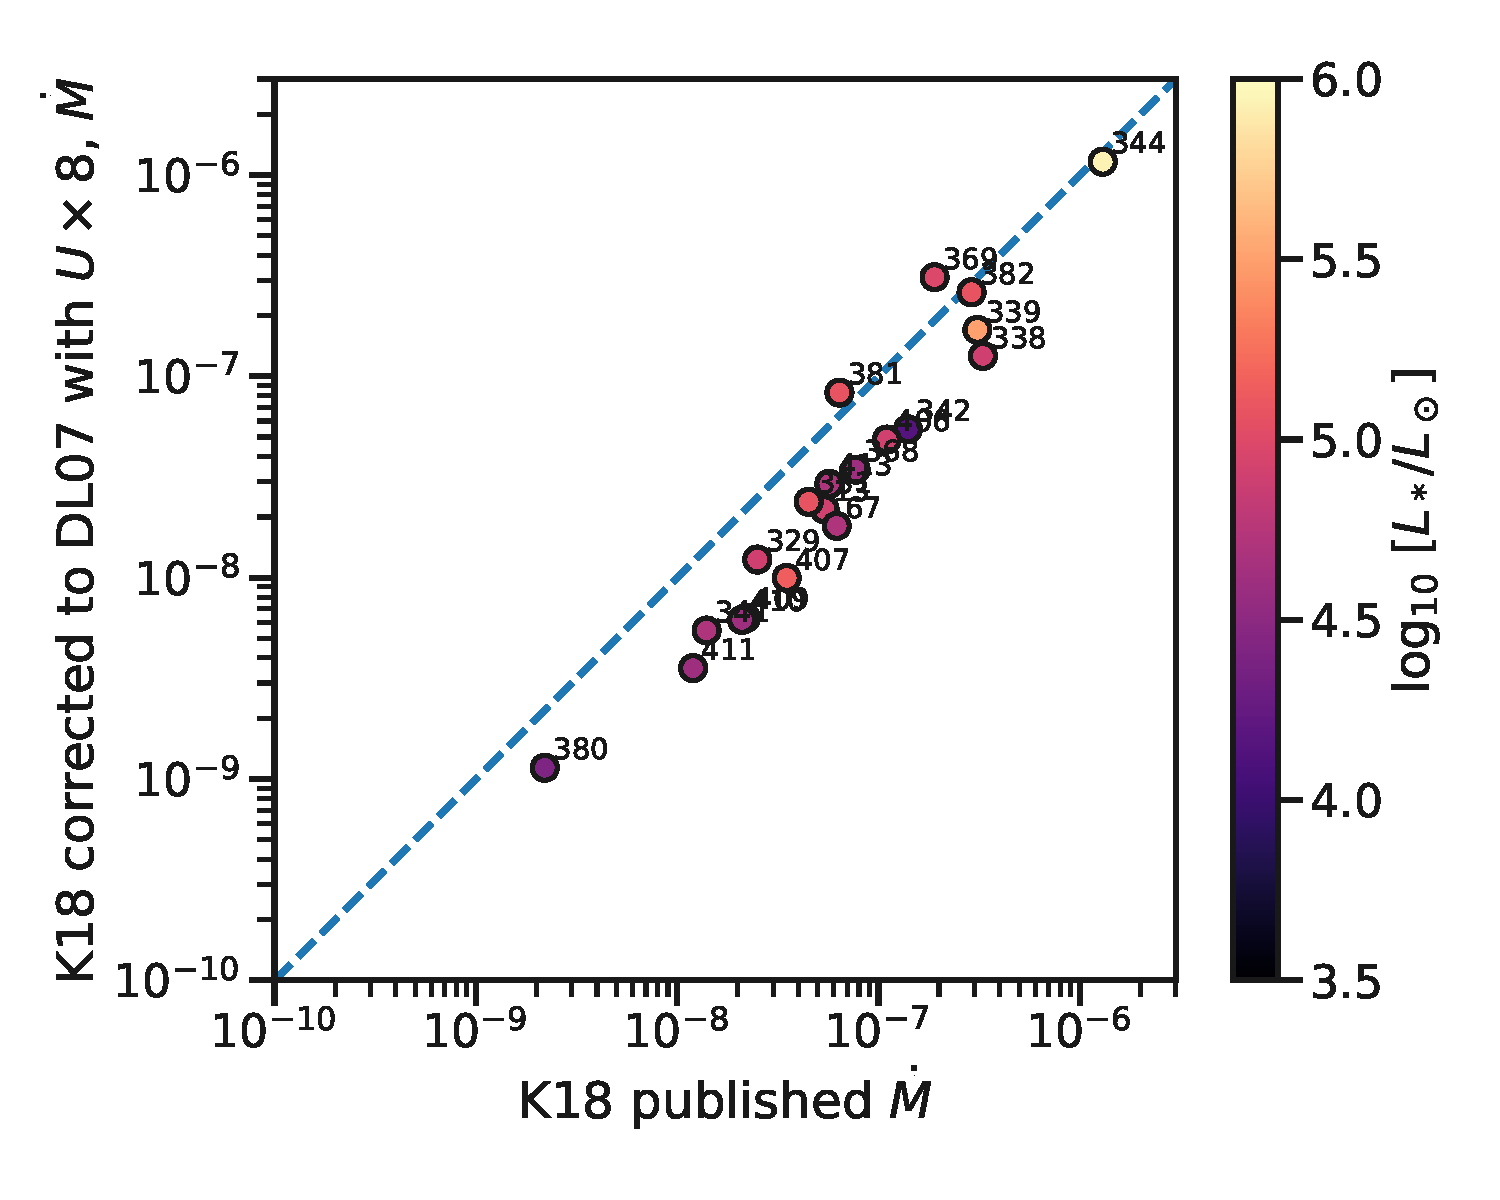
\includegraphics[width=\linewidth]{figs/K18-mdot-Ux8-comparison}
  \caption{Effects on mass-loss determination of correcting the K18
    emissivities.  The mass-loss rates from Table~2 of K18 are shown
    on the \(x\) axis, while the corrected values are shown on the
    \(y\) axis.  The corrected mass-loss rates are predominantly lower
    by a factor of roughly 2.}
  \label{fig:k18-mdot-corrected-emissivity}
\end{figure}

\begin{figure}
  \centering
  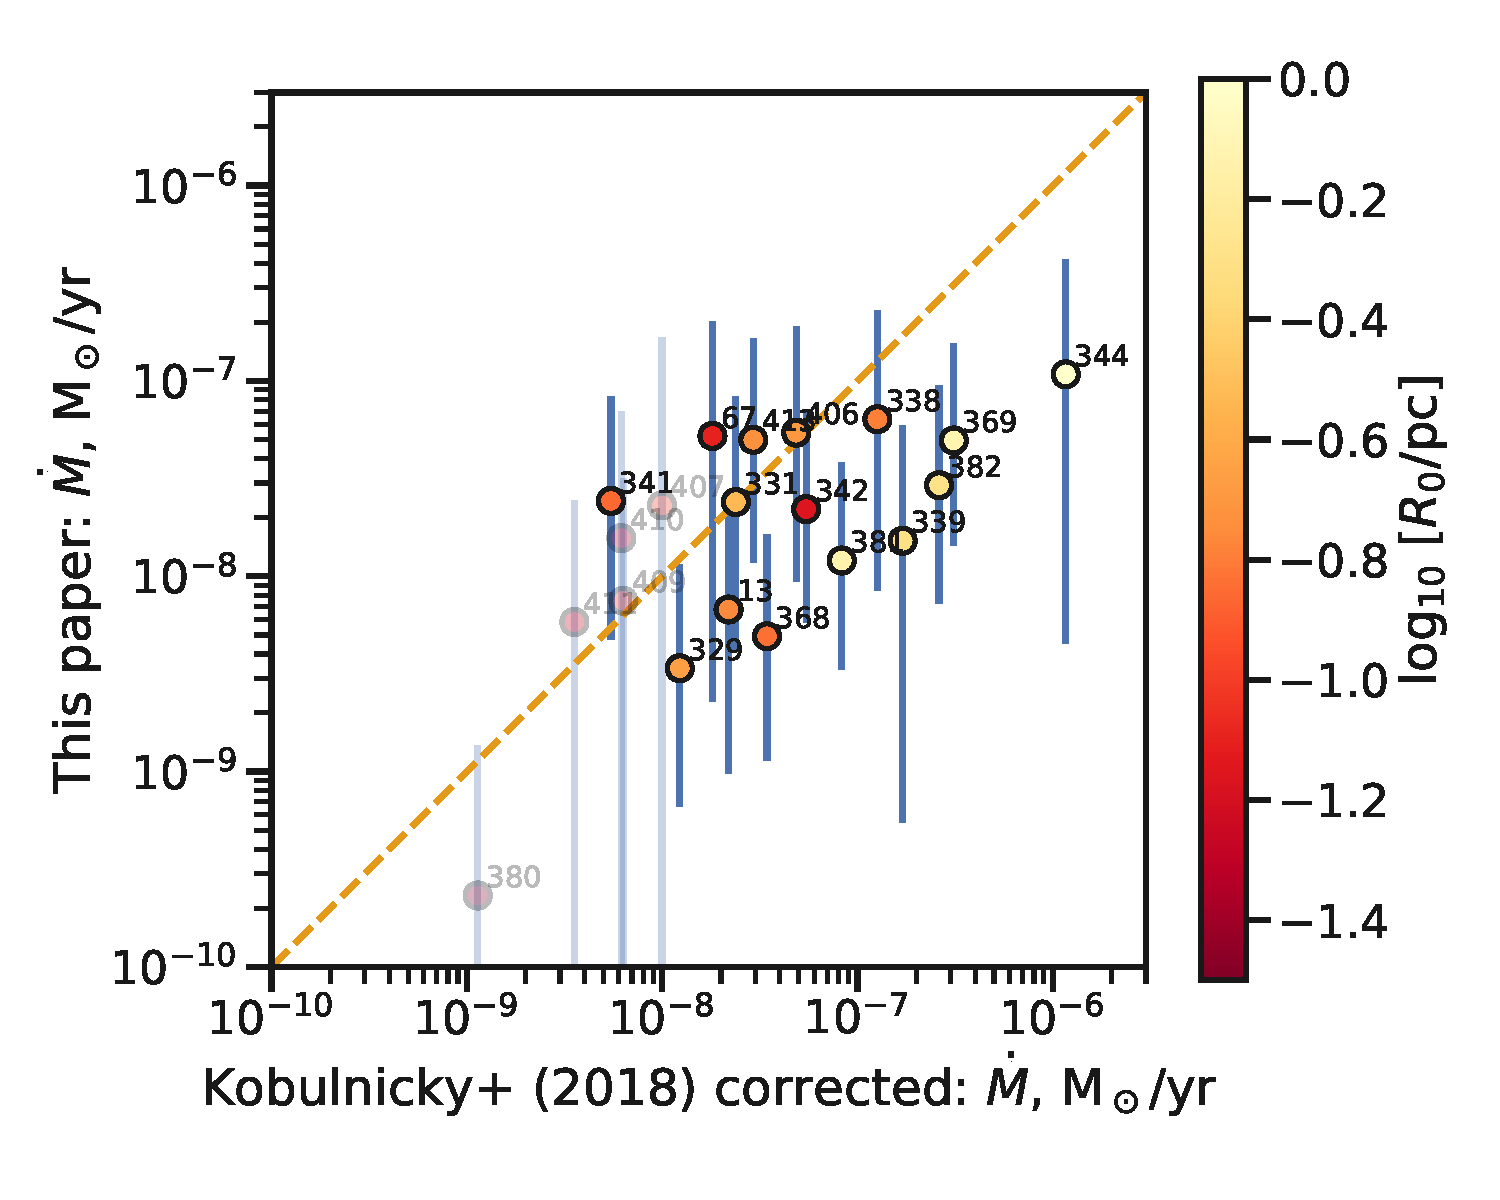
\includegraphics[width=\linewidth]{figs/K18-mdot-corrected-comparison-R0}
  \caption{Comparison of two mass-loss methods.}
  \label{fig:mass-loss-comparison}
\end{figure}


%%% Local Variables:
%%% mode: latex
%%% TeX-master: "dusty-bow-wave"
%%% End:
